\documentclass{extarticle}
\usepackage{etex}
%\usepackage[7pt]{moresize}
%\fontfamily{<familyname>}\selectfont
\renewcommand{\sfdefault}{phv}
\usepackage{anyfontsize}
\usepackage{textcomp}
\usepackage{multirow}
\usepackage{standalone}
\usepackage{verbatim}
\usepackage{authblk}
\usepackage{graphicx}
\usepackage{graphics}
\usepackage{multicol}
\usepackage{indentfirst}
\usepackage{pstricks,pstricks-add,pst-math,pst-xkey}
\usepackage{amsmath}
\usepackage{algorithm}
\usepackage[noend]{algpseudocode}
\usepackage{float}
\usepackage{filecontents}
%Lettres françaises
\usepackage[cyr]{aeguill}
\usepackage[francais]{babel}
\usepackage[T1]{fontenc}    %% permet d'utiliser les caractères accentués
\usepackage[utf8]{inputenc} %% permet d'utiliser les caractères accentué
%PGF plot
\usepackage{pgfplots, pgfplotstable}
\pgfplotsset{compat=newest}
\usepgfplotslibrary{statistics}
\pgfplotscreateplotcyclelist{mycolorlist}{blue,red,brown,teal,violet,cyan,green,black}
\pgfplotscreateplotcyclelist{mylegend}{Ly-a,Target,LRG,ELG,Fake,Fake,SS,SF}
\usepackage{xifthen}


%Debug box warnings
\showboxdepth=\maxdimen
\showboxbreadth=\maxdimen
%%%% debut macro %%%%
\newenvironment{changemargin}[2]{\begin{list}{}{%
\setlength{\topsep}{0pt}%
\setlength{\leftmargin}{0pt}%
\setlength{\rightmargin}{0pt}%
\setlength{\listparindent}{\parindent}%
\setlength{\itemindent}{\parindent}%
\setlength{\parsep}{0pt plus 1pt}%
\addtolength{\leftmargin}{#1}%
\addtolength{\rightmargin}{#2}%
}\item }{\end{list}}

%\begin{changemargin}{0cm}{0cm}
%\end{changemargin}

%%%% fin macro %%%%

%Bilio
\usepackage[nottoc,notlof,notlot]{tocbibind}
%Dash lines
\newcommand\Algphasee[1]{%
\Statex\hspace*{-\algorithmicindent}\textbf{#1}%
\vspace*{-.7\baselineskip}\Statex\hspace*{\dimexpr-\algorithmicindent-2pt\relax}\rule{\linewidth}{0.4pt}%
}

\newcommand\Algphase[1]{%
\vspace*{-.7\baselineskip}\Statex\hspace*{\dimexpr-\algorithmicindent-2pt\relax}\rule{\linewidth}{0.4pt}%
\Statex\hspace*{-\algorithmicindent}\textbf{#1}%
\vspace*{-.7\baselineskip}\Statex\hspace*{\dimexpr-\algorithmicindent-2pt\relax}\rule{\linewidth}{0.4pt}%
}

\makeatletter
\def\BState{\State\hskip-\ALG@thistlm}
\makeatother

\def\begeq{\begin{equation}}
\def\endeq{\end{equation}}
\def\begeqar{\begin{eqnarray}}
\def\endeqar{\end{eqnarray}}
\def\Rmm{R_{\rm mm}}
\def\Rdeg{R_{\rm deg}}
\def\micron{\mu{\rm m}}
\def\lya{Ly-$\alpha$\ }

\usepackage{geometry}
\geometry{hscale=0.85,vscale=0.85,centering}
\title{Description of fiber assignment code for Mocks in DESI experiment}
%\author{Robert Cahn and Louis Garrigue}
\author[1]{Robert N. Cahn\thanks{rncahn@lbl.gov}}
\author[2]{Louis Garrigue\thanks{louis.garrigue@ens.fr}}
\affil[1]{Department of Cosmological Physics, LBNL, Berkeley}
\affil[2]{Departement de physique, Ecole normale superieure, Paris}
\date{\today}
%--------------------------------------------------------------------------------------------
\begin{document}
\begin{titlepage}
\maketitle
\begin{center}
  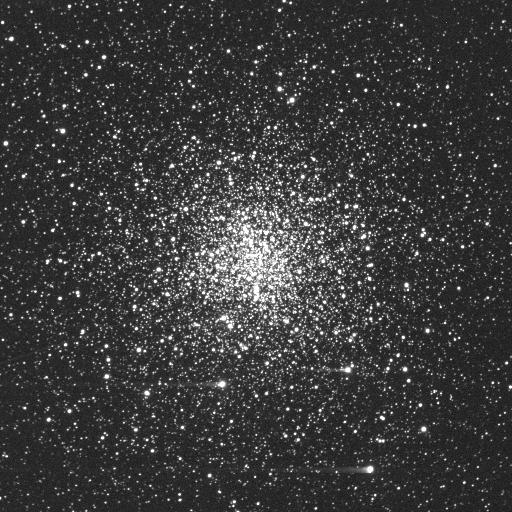
\includegraphics[width = 100mm]{figs/black.jpg}

  
\includegraphics[width = 20mm]{figs/logolbnl.png} \hfill
  \includegraphics[width = 20mm]{figs/logodesi.jpg} \hfill
  
\includegraphics[width = 20mm]{figs/logoens.png} 
\end{center}
\end{titlepage}


\begin{comment}

Dark energy study began in 1998, when two independent teams, led by Adam Riess and Saul Perlmutter, found out, using quasars measurements, that the universe was still expanding. The then standard cosmological model, which components were baryonic and dark matter ruled by general relativity, had to be changed. The $\Lambda$-CDM model now include dark energy, a component explaining the fact that gravity is weaker than expected, and compatible with the exponentially accelerating rate of the universe. It is still today the standard model. One of the main goals of cosmology is then to understand how the universe has been evolving until today, from the oldest times we can reach thanks to the Planck satellite which scrutinizes the Cosmic Microwave Background, picture of the sky 378,000 after the big bang. This study needs to understand the nature of dark energy and has to get information on the distribution of matter over time. This thus involves to scrutinize millions of galaxies and quasars, their spectrum and redshift carrying a lot of data. Such a work needs huge surveys, like BOSS, BigBOSS, and now DESI, heir of the previous ones. DESI will then significantly improve the knowledge on caracteristic features, espacially the power spectrum (Fourier transform of the correlation function of the matter density) which permits to understand baryon acoustic oscillations (BAO) which went through the early universe and which signature has always been remaining. One of the pivotal points of the DESI experiment is the assignment of its 5000 fibers on 10666 different tiles, watching galaxies in a mock catalog of 70M ones. Indeed, the efficiency of DESI will directly depend on multiple features of this assignment algorithm : number of unassigned fibers, number of times a QSO \lya will be observed (5 times goal), etc. Here is a brief presentation of the standard cosmological model and the DESI experiment. We then describe the principles used, rules, C++ code organisation and results of the assignment we created, run on the Edison NERSC Supercomputer.


\begin{multicols}{2}
\tableofcontents


	\section{Cosmology today}
\subsection{Recent breakthroughts}


	\section{Cosmology today}


	\subsection{Dark matter}
	Dark matter is invisible (doesn't react with electromagnetic radiations), and has been discovered when physicists noticed that there must be additional matter in clusters of matter. It accounts for 27\% of the totality of matter and implies that the standard model of particle physics must be incomplete. Through gravitational interaction with baryonic matter, they influence the large scale structure formation, but also small-scale clustering of galaxies lying in host dark matter halos.


	\subsection{\Lambda-CDM model}
	This is the currently standard model. It assumes that the universe is ruled by regular general relativity, and assumes the existence of dark matter and of the Einsein's cosmological constant \Lambda.
	It  respects the cosmological principle : our observational location in the Universe is not unusual or special ; on a large-enough scale, the Universe looks the same in all directions (isotropy) and from every location (homogeneity).


There is a growing consensus among cosmologists that the total density of matter is equal to the critical density, so that the universe is spatially flat. Approximately 24\% of this is in the form of a low pressure matter, most of which is thought to be “non-baryonic” dark matter, while the remaining 71\% is thought to be in the form of a negative pressure “dark energy”, like the cosmological constant. If this is true, then dark energy is the major driving force behind the fate of the universe and it will expand forever exponentially.


	\section{DESI}
	The Dark Energy Spectroscopic Instrument (DESI) is a Stage IV experiment that will make the next major advance in dark energy. \cite{Levi:2013gra}

	\subsection{Material features}
The DESI instrument, that will be installed on the Mayall telescope in Arizona, consists of a new wide-field (3.2 deg. linear field of view) corrector plus a multi-object spectrometer with up to 5000 robotically positioned optical fibers, with a resolving power of R = 5000. The fibers feed 10 three-arm spectrographs producing spectra that cover a wavelength range from 360-980 nm and have resolution of 2000-5500 depending on the wavelength. It will watch at 14,000 sq. deg. in 10666 tiles from 2018 to 2022, with roughly 7 different tiles each night.

\subsection{Aspects}
It will study baryon acoustic oscillations (BAO) and the growth of structure through redshift-space distortions. 

for targets that trace the evolution of dark energy from redshift 0.2 out to 3.5 using three kinds of celestial objects : luminous red galaxies (LRG), emission line galaxies (ELG) and quasars. 
This survey is the successor of the Stage-III BigBOSS survey and complements imaging surveys such as the Stage-III Dark Energy Survey (DES, currently operating) and the Stage-IV Large Synoptic Survey Telescope (LSST, planned start in the next decade).

On the Mayall telescope, DESI will obtain spectra and redshifts for at least 18 million emission-line galaxies, 4 million luminous red galaxies and 3 million quasi-stellar objects, in order to : i) probe the effects of dark energy on the expansion history using baryon acoustic oscillations (BAO), ii) measure the gravitational growth history through redshift-space distortions, iii) measure the sum of neutrino masses, and iv) investigate the signatures of primordial inflation. The resulting 3-D galaxy maps at z < 2 and Lyman-alpha forest at z > 2 will make 1\%-level measurements of the distance scale in 35 redshift bins. This will provide unprecedented constraints on cosmological models.


\section{Rules for fiber assignment}
We know the repartition of matter (by repartition of H matter) by pics.
The original catalog of 50M galaxies has only information on the position and the type of the galaxy, which is LRG, ELG or QSO. Those information were given by a previous survey, only based on colors, the redshift wasn't then computed. But there are different types of each one. QSO can be \lya, target or fake (actually fake ones can be stars for example). A python code generates the file of galaxies, simulating with appropriate probabilities each type, taking into account the fact that there are correlations between positions of galaxies (accordingly with BAO and gravition). When we watch at a QSO and we see that it's a fake or a target, we don't watch at it anymore. But if it's a real one, we try to see it 5 times if it is possible.
The absorption spectrum shows a pic at $\lambda = 1216$ \AA. We can deduced the redshift because we receive a wavelenght $\lambda(1+z)$. As spectrometers can only see wavelenghts in the range 380 nm (under, no enough energy is received) - 980 nm, the minimum redshift we can reach is 2.2.
At first, there was as code written by Martin White then Robert Cahn that did an assignment of tilefibers - galaxies in a global way : naive assignment, improvement (try to reassign some fibers to other ones to assign free ones) and redistribution (do not assign more, but it's to have a better repartition of free fibers on each petal).
We have to reserve 10 fibers by petal to Standard Stars and 40 to Sky Fibers.
We have to avoid unmastered correlations. That's why we don't (at first sight), when we take a new tile, associate 50 free fibers to regions of low QSO density. We would rather assign until there are only 50 free fibers left.
We do the compuation in real time. That means that we do it tile by tile. We can't access the information of all the galaxies because we only have past watched galaxies information. That adds a new constrain. So I rewrote algorithms so that they would compute an optimal assignment for one plate, knowing information on previous one assignments, and knowing information on previously watched galaxies.


\end{multicols}
\end{comment}



\begin{multicols}{2}
\section{Introduction}
Martin White developed C++ code for fiber assignment over the full 14k sq. deg. footprint.  We first modified Martin's code to incorporate features from Robert's python code, which ran on a restricted 480 sq. deg.. We included the improvement and redistribution steps, which switches fiber assignments to increase the number of galaxies observed. We then adapted the code to compute assignments not globally anymore "knowing all information on galaxies" but plate after plate, as in real experiment.
The samples are taken from Martin's mocks in stored on NERSC at /project/projectdirs/desi/mocks/preliminary/.  From these files we create a single file containing the appropriate mix of ELG, LRG, QSO, SS (Standard Stars) and SF (Sky Fibers) using the python script in git fiberassign/bin/make\_catalog\_starsandsky.py.  In the same place there is python code to produce a mixture of galaxies without any correlations, but with the correct dn/dz.  
  
  The code needs to know the locations of the positioners in the focal plane.  They are given in : \$DESIMODEL/data/focalplane/fiberpos.txt.
  It also needs to know the locations of the centers of the fields in the sky, i.e. the plates, and their order.  The original code written by Martin White provided the option of having the plate centers given in a binary file or an ASCII file.  We are now using the ASCII option by defining ASCIICENTERS at the outset.  If one wants to use the previous binary format, he has to ask it to Robert and adapt it to the new structure. The format is that of \$DESIMODEL/data/footprint/desi-tiles.par, but an alternative ASCII file can be provided. If the executable is {\tt assign} then the calling sequence will look like :
  {\tt./assign galaxies.rdzipn desi-tiles.par fiberpos.txt assignment}
 Here the catalog of targets is in the NERSC directory :
  /projects/projectdirs/desi/mocks/ preliminary/objects\_ss\_sf0.rdzipn the binary file created by {\tt make\_catalog}. The plate centers are provided here by \$DESIMODEL/data/footprint/desi-tiles.par The locations of the positioners are given in \$DESIMODEL/data/focalplane/fiberpos.txt An option not now used is to write the actual assignments to a file here called {\tt assignment}.
  
  README.rst gives instructions for running on NERSC. The problem of colliding fiber positioners is addressed in a simplified way. 
  We summarize here the various components of the code to facilitate their modification later.
Here are some features on input galaxies simulated catalog :

\begin{table}[H]\centering
	\begin{tabular}{rcccl} \hline
		Kind&Id&Priority&Nobs&Density/sq.deg.\\ \hline
		QSO Ly-$\alpha$& 0 & 1 & 5 &  50\\
		QSO Tracer & 1 & 1 & 1& 120\\
		LRG & 2 & 3 &2 & 300\\
		ELG & 3 & 5 & 1 & 2400\\
		Fake QSO & 4 & 1 & 1& 90\\
		Fake LRG & 5 & 3 & 1 & 50\\
		Standard Star & 6 & 2 & 1&  ?\\
		Sky Fiber & 7 & 4 & 1& ?\\ \hline
	\end{tabular}
	\caption{Characteristics of galaxy samples as set in make\_catalog\_rnc.py}\label{table:characteristics}
\end{table}


\section{Source files}
They all consist in a .h and a .cpp file and are in this inscreasing dependency order :
\begin{itemize} 
	\item macros : set as global some parameters of the program
	\item misc : a home-made library of structures (and functions on them) needed to manipulate concerning datas, but independent of them. There are pair (of int), List (of int), Table, Cube, and timing, printing, string conversion, error report items.
	\item structs : structures of the manipulated datas and their members
	\item global : main high-level functions and algorithms used in the program to collect information, assign fibers and print statistics. Important ones are described further
	\item main : neat and quickly understandable code that sum up all steps
\end{itemize} 

\section{Parameters}
They are defined at the begining of the file main.
\begin{itemize} 
	\item parameters sumed-up in the table \ref{table:characteristics}
	\item Npass = 5 number of passes
	\item MinUnused = 50 (not used anymore for the moment) minimum number of unused fibers on each petal
	\item MaxSS = 10 ; MaxSF = 40 maximum number of fibers assigned to SS and SF on a petal
	\item PlateRadius = 1.65 radius of the plate
	\item TotalArea = 15789.0 total scrutinised area of the sky
	\item Collide = 2.1 minimum distance allowed on plate projection of two assigned galaxies on the same plate
	\item NeighborRad = 11.0 maximum distance to consider that two fibers are neighbors
	\item PatrolRad = 6.0 maximum distance, on plate coordinates, that allows a fiber to watch at a galaxy
	\item InterPlate = 200 minimal plate distance between two plates observing the same galaxy
	\item Randomize = false randomize order of plates in making plans
\end{itemize} 


\section{Classes and structures}
They are build in order to be independent to each other, flexible, quickly understandable, in a logical way, and with no redundant information.

\end{multicols}
\begin{table}[H]\begin{center}
	\begin{tabular}{|l|l|p{12cm}|} \hline
		Structure name & Meaning & Description \\ \hline \hline

		Feat & Features of galaxies & Initialized in the main function, memories priorities, number of observations wished, and types of different galaxies.\\ \hline

		PP & Plate Parameters & Carries positions of fiber positions on the plate, spectrometer correspondence, and neighboring fibers information.\\ 

		onplate & Plate coordinates & Is used for coordinates in the focal plane in mm. The member {\tt id} is used to give the identity of a galaxy. Onplates is vector of onplate.\\ 

		plate & A plate & Peculiarly describes both the location in the sky of the tile in terms of a unit vector derived from RA and DEC. Carries also the Id of the tile, its pass, and the available galaxies it is able to reach. Then Plates is vector of plate, and has all information on tiles.\\ \hline

		galaxy & A galaxy & Information on a galaxy : an {\tt id} that corresponds to table \ref{table:characteristics}, a position in the sky (in 2 differents ways), and the available tile-fibers that can watch at it. Gals is vector of galaxy and carries all information on galaxies.\\ \hline

		Assignment & An entire assignment & Carries maping of tile-fibers to galaxies, its inverse, galaxies to tile-fibers, and the cube (3d-matrix) of assigned fibers for a kind, a petal and a plate (useful to have fast computations).\\ \hline
	\end{tabular}\end{center}
	\caption{Classes and structures}\label{tab:structures}
\end{table}
\begin{multicols}{2}

\section{Functions}
In algorithms, j stands for a plate, k for a fiber, p for a petal, g for a galaxy.

\subsection{Collecting}
{\tt collect\_galaxies\_for\_all} is multithreaded, and for each fiber of each tile, collects reachable galaxies. It uses kdTree and htmTree libraries written by Martin White, because it's absolutelly necessary to do computations in a reasonnable time with supercomputers.

{\tt collect\_available\_tilefibers} computes, using the previous work, available tile-fibers for each galaxy (inverse map)

\subsection{Useful sub-functions for global functions}
{\tt plate\_dist} turns radians into mm on the focal plane, i.e. it is the plate scale as a function of angle.

{\tt change\_coords} is a critical function that combines a galaxy and a particular plate to give the coordinates the galaxy will have in the focal plane when observed as with this tile. It's a rotation in angular coordinates. This ought to be rigorously checked.

{\tt find\_collision} returns the fiber number of a fiber that conflicts with tiblefiber (j,k).  Conflict is defined by two observed galaxies being separated by less than {\tt Collide}, currently set to 2.1 mm.

{\tt ok\_assign\_g\_to\_jk\_nobs and ok\_assign\_tot} checks to see if we can assign g to the tile-fiber (j,k), according to assigning rules described further

{\tt find\_best (j,k)} finds the best reachable galaxy for this fiber, according to assignment rules

\begin{algorithm}[H]
	\caption{Find best(j,k)}\label{euclid}
	\begin{algorithmic}[1]
		\State Initialize a fictive galaxy to -1, called best
		\For {each galaxy available galaxy (for this fiber) g}
		\If {g is better}
		\State $best \gets g$
		\EndIf
		\EndFor
	\end{algorithmic}
\end{algorithm}

{\tt assign\_fiber(j,k)} tries to assign this fiber using find\_best

{\tt improve\_fiber (j0,n,j,k)} if this fiber is unused, tries first to simply assign it, and if it doesn't work, tries to reassigning some used one (jp,kp) where $j0\le jp \le j0+n$. Before : (jp,kp) - g ; (j,k) \& gp free. After : (j,k) - g \& (jp,kp) - gp. The power of this function lies in the fact that j and jp can correspond to different passes.

\begin{algorithm}[H]
	\caption{Improve\_fiber(j0,n,j,k)}\label{euclid}
	\begin{algorithmic}[1]
		\If {k is not assigned}
		\State try to assign\_(j,k)
		\If {k couldn't just be assigned}
		\For {each available galaxy g}
		\If {it's possible to assign g with k}
		\For {each chosen tile-fibers (jp,kp) which choosed g (where $j0\le jp \le j0+n$)}
		\State $gp\leftarrow find\_best(jp,kp)$
		\If {$gp \ne -1$}
		\State Unassign $(jp,kp) \longleftrightarrow g$
		\State Assign $(j,k) \longleftrightarrow g$
		\State Assign $(jp,kp) \longleftrightarrow gp$
		\EndIf
		\EndFor
		\EndIf
		\EndFor
		\EndIf
		\EndIf
	\end{algorithmic}
\end{algorithm}


\subsection{Assigning making a plan}
Here are algorithms that know all information and are able to compute the assignment crossing between plates. It does a plan with only information available by the catalog and by previous seen galaxies. One can use them with size 1 if one wants to do an assignment plate after plate for instance (which shouldn t be called a plan anymore).

The "next" argument means that we treat (in a shuffle order) all next "next" plates (in the right order of tiles) in the plan we make. If it is $-1$, it will deal with all left plates.

{\tt simple\_assign} makes a first simple assignment plan : for each fiber assign to the best available galaxy

\begin{algorithm}[H]
	\caption{Simple\_assign(j0,n)}\label{euclid}
	\begin{algorithmic}[1]
		\For {each plate j from j0 to j0+n in a random order}
		\For {each fiber k in a random order}
		\State try to assign\_fiber(j,k)
		\EndFor
		\EndFor
	\end{algorithmic}
\end{algorithm}

{\tt new\_assign\_fibers} makes a first assignment plan trying to assign only QSO, then ELG and LRG, then trying to assign SF and SS replacing other kinds if there are not enough available fibers. This way, a QSO could can't be lost because of a collision. With the current value of Collision, it's not very useful, but could be for bugger values.

\begin{algorithm}[H]
	\caption{New\_assign\_fibers(j0,n)}\label{euclid}
	\begin{algorithmic}[1]
		\For {each plate j from j0 to j0+n in a random order}
		\For {each petal p of this plate, in a random order}
		\For {each fiber k of this petal, in a random order}
		\State Try assign\_fiber(j,k) only allowing QSO
		\EndFor
		\For {each fiber k of this petal, in a random order}
		\State Try assign\_fiber(j,k) only allowing ELG and LRG
		\EndFor
		\For {each unassigned fiber k of this petal}
		\State Try assign\_fiber(j,k) to only SS or SF
		\EndFor
		\If {Number of SS $\le$ 10}
		\State Replace ELG (then LRG) to an SS until there are 10 SS
		\EndIf
		\If {Number of SF $\le$ 40}
		\State Replace ELG (then LRG) to an SF until there are 40 SF
		\EndIf
		\EndFor
		\EndFor
	\end{algorithmic}
\end{algorithm}

{\tt improve} improves the plan applying improve\_fiber to all of the fibers that concern it

{\tt improve\_from\_kind (kind)} for every petal, tries to assign unassigned fibers to SS or SF, to release an other fiber (formerly assigned to a SS or SF) that would be reassigned to a regular galaxy (kind is SS or SF when we call it)

\begin{algorithm}[H]
	\caption{Improve\_from\_kind (kind,j0,n)}\label{euclid}
	\begin{algorithmic}[1]
		\For {each plate j from j0 to j0+n in a random order}
		\For {each petal p of this plate, in a random order}
		\For {each unassigned fiber k}
		\For {each available galaxies g of k}
		\For {each fiber kp of p assigned to a galaxy of kind}
		\If {no conflict}
		\State Reassign kp to g
		\State Assign k to a galaxy of kind kind
		\EndIf
		\EndFor
		\EndFor
		\EndFor
		\EndFor
		\EndFor
	\end{algorithmic}
\end{algorithm}

{\tt update\_plan\_from\_one\_obs} updates the plan formerly made so that if for example on the previous observation we've watched at a fake QSO, it won't be observed anymore in case it was planed to be observed once or several times again. Released tile-fibers will then be tryed to be reassigned with improve\_fiber

\begin{algorithm}[H]
	\caption{Update\_plan\_from\_one\_observation(j0,end\_plan)}\label{euclid}
	\begin{algorithmic}[1]
		\State get the list of galaxies watched by this plate that are discovered fake or target
		\For {each of those galaxies g}
		\State get the list of planed tile-fibers watching this galaxy further in the plan $j0\le jp \le end$
		\For {each of those tile-fibers (jp,kp)}
		\State Unassign $(jp,kp) \longleftrightarrow g$
		\State run improve\_fiber(j0+1,end-j0,jp,kp)
		\EndFor
		\EndFor
	\end{algorithmic}
\end{algorithm}


\subsection{Displaying results}
{\tt results\_on\_inputs} displays some statistics on treated input files (recall input features, print statistics on the number of fibers with 0 galaxies within reach, 1 galaxy within reach etc. out to 19 galaxies within reach ; number of available tile-fibers for a galaxy, ...)

{\tt display\_results} writes some statistics and provides the tex-formatted results to make Table \ref{tab:full14k}

{\tt print\_free\_fibers} print histograms on free fibers towards/regarding petals, for everything, for only SS and for only SF


\subsection{Other not used anymore functions}
They are redistribution function (redistribution of galaxies (simply or by kind), tile-fibers) used in previous development of the program. We let them here because they can be useful for further develop,ent of the code (redistributing assignment can add new degrees of freedom for an other improvement function execution for example).


\section{Rules of assignment}
\begin{itemize}
	\item of course, a tile-fiber is only assigned once
	\item a galaxy can't be assigned more than once in a pass
	\item two observed galaxies can't be separated by less than {\tt Collide} (set by find\_collision)
	\item in last pass, only ELG, SS and SF are scrutinised
	\item there can't be more than 10 fibers assigned to SS on a petal
	\item there can't be more than 40 fibers assigned to SF on a petal
	\item basically, we choose best galaxy from at the same time available, watched less than maxgoal(kind) times and unassigned ones. Amongst them, we take those which has the least priority, and then the one which has been seen the least number of times
\end{itemize}

In reality we only know the basic type (QSO, LRG, ELG, SS, SF) of the galaxies of the catalog. The precise type is only infered by a simulation coded in python, but is generated with randomness. So in the algorithms, we can know the nature of the object only when it has been watched once at least.
There are two way of assignment : either watch tile after tile and foresee the assignment of the tile just before watching it ; otherwise, we can make a plan for a definite number of next tiles. In such a plan, we try to optimize assignment, but of course, we can't know the precise type (fake, ...) so it is possible to foresee to observe for example 4 times a fake QSO. We won't do it, so after having planed, when we begin to apply it and do the real observation, if we have just previously observed a fake QSO, we will remove further observations in this plan. We then try to assign the released tile-fibers. In the code, a difficulty was optimization at this point : we could have replaned everything in the plan after an update of information, but we can't because that would take too much time. So we only try to reassign released tile-fibers.

The idea is to get most information possible in the first pass, assigning independently tile after tile, and then, after this first pass, make a plan for everything else, when we have information on most of the QSO and LRG (the only kinds we want to observe several times). The plan will be better that way, because we do less mistakes than if we would do it from the begining.


\section{Algorithm}

The calling sequence is {\tt assign galaxy plate\_centers fiberpos assignment}. The last of these is the file to which we would write all the final galaxy assignments, but this is generally suppressed since we aren't using it yet.

 {\tt main} proceeds by taking important parameters, features of galaxies, reading in the galaxies to make G, the positions of the fibers on the plate to make pp, the plate centers and positioner locations to make P. 
 
We then collect available galaxies for each fiber for each plate, and compute the inverse map.
 
We next, tile after tile, do the assignment of galaxies. We have tried several strategies : making several plans, use simple assignment, use complexe one, improve several times, in several ways, etc... Here is the one which gives the best results.

We present the strategy that produced the best results, which will be the strategy of reference,
We tried a strategy where we make then apply a plan for the first 2000, then for the following 2000, then for the left, but it's not better.

Simple assign fibers and new assign, even if there structure are quite different, give almost the same results. Simple assign is a little bit quicker so we will use this one.

\begin{algorithm}[H]
	\caption{Assignment of reference in main program}\label{euclid}
	\begin{algorithmic}[1]
		\Algphasee{Phase I - Make a plan for the first 2000 plates}
		\State Run, globally, on the list plates from 0 to 1999 :
		\State Assign fibers
		\State Improve SF
	\end{algorithmic}
	\begin{algorithmic}[1]
		\Algphase{Phase II - Applying the plan}
		\For {each plate j of the plan, in order}
		\State Real observation is here
		\State Update information collected on previous just watched tile
		\State Update\_plan\_from\_one\_observation(j)
		\EndFor
	\end{algorithmic}

	\begin{algorithmic}[1]
		\Algphase{Phase III - Make a plan for all left plates}
		\State Run, globally, on the list plates from 2000 to the end :
		\State Assign fibers
		\State Improve
		\State Improve SF
		\State Improve SS
		\State Redistribute
		\State Improve
		\State Redistribute
		\State Improve
	\end{algorithmic}

	\begin{algorithmic}[1]
		\Algphase{Phase IV - Applying the plan}
	\end{algorithmic}
\end{algorithm}


A standard output display of an execution look like that (for assignment plan and applying):
{\tt \small 

 - Plate 1998 :      9 not as -     0 unas \&    0 replaced

 - Plate 1999 :      8 not as -     0 unas \&    0 replaced

\# ... took : 10.5 s

\# Begin simple assignment :

  37,635,165 assignments on all left next plates

\# ... took : 2 mn 17.3 s

\# Begin improve :

  921,594 more assignments (2.449 \% improvement)

\# ... took : 42.1 s

\# Begin improve SF :

  1,386,726 more assignments (3.597 \% improvement)

\# ... took : 3 mn 13.8 s

\# Begin improve SS :

  194,603 more assignments (0.487 \% improvement)

\# ... took : 6.99 s

\# Begin redistribute TF :

  2,202,483 redistributions of couples of TF

\# ... took : 16.8 s

\# Begin improve :

  167,146 more assignments (0.416 \% improvement)

\# ... took : 23.3 s

\# Begin redistribute TF :

  2,058,702 redistributions of couples of TF

\# ... took : 16.8 s

\# Begin improve :

  76,484 more assignments (0.190 \% improvement)

\# ... took : 22.1 s

\# Begin real time assignment at 11 mn 34.7 s

 - Plate 2000 : SF-imp + 38 (+0.769 \%) SS-imp +  1 (+0.020 \%)    22 not as -  2630 unas \& 1985 replaced

 - Plate 2001 : SF-imp + 37 (+0.750 \%) SS-imp +  1 (+0.020 \%)    29 not as -  3227 unas \& 2619 replaced

 - Plate 2002 : SF-imp + 34 (+0.691 \%) SS-imp +  2 (+0.040 \%)    44 not as -  3296 unas \& 2632 replaced

 - Plate 2003 : SF-imp + 13 (+0.262 \%) SS-imp +  1 (+0.020 \%)    17 not as -  2797 unas \& 2526 replaced
}

\section{Results}
\subsection{Results on the input catalog}
Here are some statistics on the input galaxies catalog :

\begin{figure}[H]\begin{center}
	\begin{tikzpicture}[scale=1.1]\begin{semilogyaxis}[const plot,enlarge x limits=false,xmax=10,xlabel={\# of accessible galaxies},ylabel={},cycle list name=mycolorlist,legend entries={QSO \lya,QSO Tracer,LRG,ELG,Fake QSO,Fake LRG}] 
		\addplot table[x=x,y=0] {figs/avgalhist.dat};
		\addplot table[x=x,y=1] {figs/avgalhist.dat};
		\addplot table[x=x,y=2] {figs/avgalhist.dat};
		\addplot table[x=x,y=3] {figs/avgalhist.dat};
		\addplot table[x=x,y=4] {figs/avgalhist.dat};
		\addplot table[x=x,y=5] {figs/avgalhist.dat};
\end{semilogyaxis}\end{tikzpicture}
\end{center}\caption{Available galaxies (by kind) for a single fiber on a single tile}\end{figure}


\begin{figure}[H]\begin{center}\begin{tikzpicture}[scale=1.1]\begin{semilogyaxis}[const plot,enlarge x limits=false,xlabel={\# of TF that can access a given galaxy},xmax=13,ylabel={},cycle list name=mycolorlist,legend entries={QSO \lya,QSO Tracer,LRG,ELG,Fake QSO,Fake LRG},legend pos=south west]
		\addplot table[x=x,y=0] {figs/avtfhist.dat};
		\addplot table[x=x,y=1] {figs/avtfhist.dat};
		\addplot table[x=x,y=2] {figs/avtfhist.dat};
		\addplot table[x=x,y=3] {figs/avtfhist.dat};
		\addplot table[x=x,y=4] {figs/avtfhist.dat};
		\addplot table[x=x,y=5] {figs/avtfhist.dat};
\end{semilogyaxis}\end{tikzpicture}\caption{Available tile-fibers for a galaxy (by kind)}\end{center}\end{figure}


\subsection{Results of the assignment}
We run the program with all information (prior knowledge of information on fake, target, etc) to compare with realistic simulation, this result is interesting.

The results are then written using {\tt display\_results}, and each assignment/improvement function display its own statistics.

 and from it, we change parameters to see the effects of them on the program. We also compare to other strategies. The best strategy (discovered until now) is the one where is the strategy where we first look at 2000 tiles, tile after tile runing simple\_assign on each tile without plan, and we then do a plan for all left tiles.

In the second plan, we can experimentally see that after a first SF-improvement ($+\sim 3.6\%$), even if we redistribute, a second one is almost useless ($+\sim 0.1\%$), whereas a second simple-improve is still efficient after a redistribution ($+\sim 0.4\%$), but useless without a redistribution step ($+\sim 0.01\%$). An other kind of kind-improvement (instead of SF and SS ($+\sim 0.5\%$)) is also almost useless. Furthermore, the computation time is far bigger for SF-improvement (5 mn) than for other.

The most results-sensible feature in it is the number of plan/applying and their plates sets. One could try to find a better one.

\end{multicols}

\subsection{Sum-up of assigned galaxies}
In the reference strategy, we have 50,095,513 assignments in total (93.94\% of all fibers). The weighted score of a certain kind is defined as : 
\vspace{1\baselineskip}
$Score(kind) = 100\cdot \frac{\sum\nolimits_{g \in kind} obs(g)}{\sum\nolimits_{g \in kind} goal}$ where $obs(g)$ is the number of times g is observed.

\begin{table}[H]\begin{center}
\begin{tabular}{r|rrrrrrrcc}
	~   &         0 &         1 &       2 &      3 &      4 &     5 &         Total &  observed $\%$ & weighted $\%$ \\ \hline
	QSO \lya   &    22,915 &   414,720 & 238,413 & 75,600 & 28,497 & 8,498 &   788,643 & 98.922 & 67.670\\ 
	QSO Tracer & 1,874,187 &    20,433 &       0 &      0 &      0 &     0 & 1,894,620 & 98.921 & 98.921\\ 
	LRG        & 3,909,020 &   562,287 & 245,036 &      0 &      0 &     0 & 4,716,343 & 94.804 & 88.843\\ 
	ELG        &29,680,067 & 8,392,913 &       0 &      0 &      0 &     0 &38,072,980 & 77.955 & 77.955\\ 
	Fake QSO   & 1,405,670 &    15,342 &       0 &      0 &      0 &     0 & 1,421,012 & 98.920 & 98.920\\ 
	Fake LRG   &   753,871 &    35,579 &       0 &      0 &      0 &     0 &   789,450 & 95.493 & 95.493\\ 
	SS         & 1,066,600 & 1,143,862 &       0 &      0 &      0 &     0 & 2,210,462 & 48.252 & 48.252\\ 
	SF         & 4,266,400 &17,838,234 &       0 &      0 &      0 &     0 &22,104,634 & 19.300 & 19.300\\ 
\end{tabular}
\caption{Remaining observations (id on lines, nobs left on rows) with total}
\label{tab:full14k}
\end{center}
 \end{table}

\begin{multicols}{2}

\subsection{Free fibers}
Here is the histogram of petals as a function of free fibers.
\begin{figure}[H]\begin{center}\begin{tikzpicture}[scale=1.1]\begin{semilogyaxis}[const plot,enlarge x limits=false,xlabel={\# of free fibers},ylabel={},xmax=160] 
	\addplot [mark=none] table [x=x,y=0] {figs/freefib.dat};
\end{semilogyaxis}\end{tikzpicture}\caption{\# of petals with that many free fibers}
\end{center}\end{figure}
 

\subsection{Redistribution-Improvement step}
We see, in the second plan, what is the effect of several redistribution-improvement executions. Here is presented the number of redistributions, number of additionnal assignments, with the improvement in \% and the total time taken for until this step.

\begin{table}[H]\centering
	\begin{tabular}{c|cccc}
		Step & \# red & \# +as & + \% & Time \\ \hline
		1 & 2,204,977 & 167,741 & .418 & 40s\\
		2 & 2,060,851 & 76,509 & .190 & 1mn 20s\\
		3 & 1,965,994 & 19,273 & 0.048 & 2mn\\
		4 & 1,945,418 & 10,738 & 0.027 & 2mn 40s\\
		5 & 1,929,917 & 7,999 & 0.020 & 3mn 20s\\
		6 & 1,921,331 & 5,745 & 0.014 & 4mn\\
	\end{tabular}
\end{table}

\begin{figure}[H]\begin{center}
\begin{tikzpicture}[scale=1.1]
	\begin{axis}[const plot,stack plots=y,enlarge x limits=false,enlarge y limits=false,xlabel={Number of available TF},ylabel={},cycle list name=mycolorlist,legend entries={0,1,2,3,4,5}]
		\addplot [fill,fill opacity=0.5,color=blue] table[x=x,y=0] {figs/obsly.dat};
		\addplot [fill,fill opacity=0.5,color=red] table[x=x,y=1] {figs/obsly.dat};
		\addplot [fill,fill opacity=0.5,color=brown] table[x=x,y=2] {figs/obsly.dat};
		\addplot [fill,fill opacity=0.5,color=teal] table[x=x,y=3] {figs/obsly.dat};
		\addplot [fill,fill opacity=0.5,color=violet] table[x=x,y=4] {figs/obsly.dat};
		\addplot [fill,fill opacity=0.5,color=black] table[x=x,y=5] {figs/obsly.dat};
	\end{axis}
\end{tikzpicture}
\caption{\# of QSO Ly-$\alpha$ (with their number of observation) as a function of available tile-fibers}
\end{center}\end{figure}


\begin{figure}[H]\begin{center}
	\begin{tikzpicture}[scale=1.1]
		\begin{semilogyaxis}[const plot,enlarge x limits=false,xlabel={},ylabel={},cycle list name=mycolorlist]
			\addplot table[x=x,y=0] {figs/dist2ly.dat};
		\end{semilogyaxis}
	\end{tikzpicture}
	\caption{Histogram of distances (in number of plates) between two consecutive observed QSO Ly-$\alpha$}
\end{center}\end{figure}


\begin{figure}[H]\begin{center}
	\begin{tikzpicture}[scale=1.1]
		\begin{axis}[const plot,enlarge x limits=false,enlarge y limits=false,xlabel={Plate},ylabel={},cycle list name=mycolorlist]
			\addplot table[x=x,y=0] {figs/fft.dat};
		\end{axis}
	\end{tikzpicture}
	\caption{Free fibers as a function of time (plates)}
\end{center}\end{figure}


\begin{figure}[H]\begin{center}
\begin{tikzpicture}[scale=1.1]
	\begin{axis}[enlarge y limits=false,enlarge x limits=false,xlabel={Plate},ylabel={},cycle list name=mycolorlist,legend entries={QSO \lya,QSO Tracer,LRG,ELG,Fake QSO,Fake LRG},legend pos=south east]
		\addplot table[x=x,y=0] {figs/time.dat};
		\addplot table[x=x,y=1] {figs/time.dat};
		\addplot table[x=x,y=2] {figs/time.dat};
		\addplot table[x=x,y=3] {figs/time.dat};
		\addplot table[x=x,y=4] {figs/time.dat};
		\addplot table[x=x,y=5] {figs/time.dat};
	\end{axis}
\end{tikzpicture}
\caption{Observed galaxy kind as a function of time (plates seen)}\end{center}\end{figure}

Besides, we have indeed exactly 10 SS and 40 SF per petal.

\begin{figure}[H]\begin{center}
	\begin{tikzpicture}[scale=1.1]
		\begin{axis}[enlarge x limits=false,xlabel={Collide (mm)},ylabel={},cycle list name=mycolorlist]
			\addplot [mark=x] coordinates {(0,68.572)(1,68.414)(1.8,67.963)(2.0,67.774)(2.1,67.670)(2.2,67.545)(2.4,67.278)(2.8,66.606)(3,66.187)(3.2,65.741)};
			\draw [densely dashed] (axis cs:2.1,\pgfkeysvalueof{/pgfplots/ymin}) -- (axis cs:2.1,\pgfkeysvalueof{/pgfplots/ymax});
		\end{axis}
	\end{tikzpicture}
	\caption{Weighted \% of \lya observed as a function of required stay-clear}
\end{center}\end{figure}

\begin{figure}[H]\begin{center}
	\begin{tikzpicture}[scale=1.1]
		\begin{axis}[enlarge x limits=false,xlabel={Collide (mm)},ylabel={},cycle list name=mycolorlist]
			\addplot [mark=x] coordinates {(0,78.301)(1,78.073)(1.8,77.999)(2.0,77.970)(2.1,77.955)(2.2,77.937)(2.4,77.894)(2.8,77.777)(3,77.703)(3.2,77.612)};
			\draw [densely dashed] (axis cs:2.1,\pgfkeysvalueof{/pgfplots/ymin}) -- (axis cs:2.1,\pgfkeysvalueof{/pgfplots/ymax});
		\end{axis}
	\end{tikzpicture}
	\caption{\% of ELG observed as a function of required stay-clear}
\end{center}\end{figure}

\begin{figure}[H]\begin{center}
	\begin{tikzpicture}[scale=1.1]
		\begin{axis}[enlarge x limits=false,xlabel={InterPlate},ylabel={},cycle list name=mycolorlist]
			\addplot [mark=x] coordinates {(1,70.172)(20,68.022)(50,67.961)(100,67.905)(200,67.670)(400,67.461)(1000,66.888)(2000,65.660)};
			\draw [densely dashed] (axis cs:200,\pgfkeysvalueof{/pgfplots/ymin}) -- (axis cs:200,\pgfkeysvalueof{/pgfplots/ymax});
		\end{axis}
	\end{tikzpicture}
	\caption{\% of \lya observed as a function of required minimum interval between plates observing the \lya}
\end{center}\end{figure}


\begin{comment}
\end{comment}


\section{Possible improvements}
We havn't tried all possible strategies, so it is possible that an other combination of runing of the functions could lead to better results.
One could also try to search for an "orthogonal" (of the 3 other ones) improvement function.
To make plans, we could use an automaton, which would be automatically able to use all kinds of assigment/improvement functions, and would go through all fibers at random to assign/improve randomly, and the controlable parameter would only be the time we want it to work.
Nevertheless, a lot of efforts now lead to little improvements of the results. It is likely that we are almost at the global optimum. We only have a doubt on the number of plans/applying and their sets of plates that could improve significantly.

\bibliographystyle{plain}
\bibliography{papers}{}

\end{multicols}
\end{document}
